\chapter{A systematic literature review of the Prisoner's Dilemma.}\label{chapter:literature_review}

\section{Introduction}

Chapter~\ref{chapter:introduction} introduced the Prisoner's Dilemma as the main
game theoretic model that will be used throughout this thesis, and presented a
brief literature review of the research this thesis is building upon. This
Chapter provides a more detailed systematic literature on the Prisoner's
Dilemma. The aim of this Chapter is to provide a concrete summary of the
existing literature and to contribute to research question 1. This is
achieved by partitioning the literature in five different sections each
reviewing a different aspect of research. The Chapter is structured as follows:

\begin{itemize}
    \item section~\ref{section:origin} presents the origin of the PD
    and reviews the early publications in the field and the use of
    human subject research.
    \item section~\ref{section:intelligent_design} presents the pioneering computer
    tournaments of Robert Axelrod and reviews IPD strategies of intelligent design.
    \item section~\ref{section:evolutionary_dynamics} discusses
    the emergence, or not, of cooperative behaviour in evolutionary dynamics.
    \item section~\ref{section:structured_strategies} defines structured
    strategies in the IPD, the notion of training and discusses related papers.
    \item section~\ref{section:software} reports on educational and research software
    used for simulating the PD game.
\end{itemize}

\section{Origins of the prisoner's dilemma}\label{section:origin}

The origin of the PD goes back to the 1950s in early experiments conducted at
RAND~\cite{Flood1958} to test the applicability of games described
in~\cite{VonNeumann1944}. The game received its name later the same year.
According to~\cite{Tucker1983}, Albert W. Tucker (the PhD supervisor of John
Nash~\cite{Nash1951}), in an attempt to deliver the game with a story during a
talk described the players as prisoners and the game has been known as the
Prisoner's Dilemma ever since.

The early research on the IPD was limited. The only source of
experimental results was through human subject research where pairs of
participants simulated plays of the game, and human subject research had
disadvantages. Humans could behave randomly and in several experiments both the
size and the background of the individuals were different, thus comparing
results of two or more studies became difficult.

The main aim of these early research experiments was to understand how
conditions such as the gender of the participants~\cite{Evans1966, Lutzker1961,
Mack1971}, the physical distance between the participants~\cite{Sensenig1972}, the
effect of their opening moves~\cite{Tedeschi1968} and even how the experimenter, by varying
the tone of their voice and facial expressions~\cite{Gallo1968}, could influence
the outcomes and subsequently the emergence of cooperation. An early figure that
sought out to understand several of these conditions was the mathematical
psychologist Anatol Rapoport. The results of his work are summarised
in \cite{rapoport1965}.

Rapoport was also interested in conceptualising strategies that could promote
international cooperation. Decades later he would submit the winning strategy
(Tit for Tat) of the first computer tournament, run by Robert Axelrod.
These tournaments and several strategies that were designed by researchers, such
as Rapoport, are introduced in the following section.

\section{Axelrod's tournaments and intelligently designed strategies}
\label{section:intelligent_design}

As discussed in Section~\ref{section:origin}, before 1980 a great deal of
research was done in the field, however, as described in~\cite{Axelrod2012}, the
political scientist Robert Axelrod believed that there was no clear answer to the
question of how to avoid conflict, or even how an individual should play the
game. Combining his interest in artificial intelligence and political science
Axelrod created a framework for exploring these questions using computer
tournaments and made the study of cooperation of critical interest. As
described in~\cite{Rapoport2015}, ``Axelrod's new approach has been extremely
successful and immensely influential in casting light on the conflict between an
individual and the collective rationality reflected in the choices of a
population whose members are unknown and its size unspecified, thereby opening a
new avenue of research''.

% In a collaboration with a colleague, Douglas Dion,
% Axelrod in~\cite{Axelrod1988} summarized a number of works that were immediately
% inspired from the ``Evolution of Cooperation''

The first reported computer tournament took place in 1980~\cite{Axelrod1980a}. 
Axelrod asked researchers to design a strategy with the purpose of winning an IPD
tournament. A
total of 13 strategies were submitted, written in the programming languages
Fortran or Basic. Each competed in a 200 turn match against all 12 opponents,
itself and a player that played randomly (called \textit{Random}). This type of
tournament is referred to as a \textit{round robin}. The tournament was repeated 5 times
to get a more stable estimate of the scores for each pair of play.
Each participant knew the exact number of turns and had access to the full
history of each match. Furthermore, Axelrod performed a preliminary tournament
and the results were known to the participants. This preliminary tournament is
mentioned in~\cite{Axelrod1980a} but no details were given.

The winner of the tournament was determined by the total average score and not
by the number of matches won. The strategy that was announced the winner was the
strategy submitted by Rapoport, \textit{Tit For Tat}. The success of Tit for Tat
came as a surprise. It was not only the simplest submitted strategy, it would
always cooperates on the first round and then mimic the opponent's previous
move, but it had also won the tournament even though it could never beat
any player it was interacting with.

In order to further test the results Axelrod performed a second tournament
in 1980~\cite{Axelrod1980b}. The second tournament received much more attention
and had a total of 62 entries. The participants knew the results of the previous
tournament and the rules were similar with only a few alterations. The
tournament was repeated 5 times and the length of each match was not known to
the participants. Axelrod intended to use a fixed probability (refereed to as
`shadow of the future'~\cite{Axelrod1988}) of the game ending on the next move.
However, 5 different number of turns were selected for each match 63, 77, 151,
308 and 401, such that the average length would be around 200 turns.

Nine of the original participants competed again in the second tournament. Two
strategies that remained the same were Tit For Tat and \textit{Grudger}. Grudger
is a strategy that will cooperate as long as the opponent does not defect,
submitted by James W. Friedman. The name Grudger was give to the strategy
in~\cite{Li20141}, though the strategy goes by many names in the literature such
as, Spite~\cite{Beaufils1997}, Grim Trigger~\cite{Banks1990} and
Grim~\cite{Van2015}. New entries in the second tournament included \textit{Tit
for Two Tats} submitted by John Maynard Smith and \textit{KPavlovC}. KPavlovC,
is also known as Simpleton~\cite{rapoport1965}, introduced by Rapoport or just
Pavlov~\cite{Nowak1993}. The strategy is based on the fundamental behavioural
mechanism win-stay, lose-shift. Pavlov is heavily studied in the literature and
similarly to Tit for Tat it is used in tournaments today and has
had many variants trying to build upon it's success, for example
\textit{PavlovD} and \textit{Adaptive Pavlov}~\cite{Li2007}.

Despite the larger size of the second tournament none of the new entries managed
to outperform the simpler designed strategy. The winner was once again Tit for
Tat. Axelrod deduced the following guidelines for a strategy to perform well:

\begin{itemize}
    \item The strategy would start of by cooperating.
    \item It would forgive it's opponent after a defection.
    \item It would always be provoked by a defection no matter the history.
    \item It was simple.
\end{itemize}

The success of Tit for Tat, however, was not unquestionable. Several papers
showed that stochastic uncertainties severely undercut the effectiveness of
reciprocating strategies and such stochastic uncertainties have to be expected
in real life situations~\cite{Milinski1987}. For example, in~\cite{Molander1985}
it is
proven that in an environment where \textit{noise} (a probability that a
player's move will be flipped) is introduced two strategies playing Tit for Tat
receive the same average payoff as two Random players.
Hammerstein, pointed out that if by mistake, one of two
Tit for Tat players makes a wrong move, this locks the two opponents into a
hopeless sequence of alternating defections and cooperations~\cite{Hammerstein1984}.
The poor performance of the strategy in noisy environments was also demonstrated
in tournaments. In~\cite{Bendor1991, Donninger1986} round robin
tournaments with noise were performed, and Tit For Tat did not win.
The authors concluded that to overcome the noise more generous strategies
than Tit For Tat were needed. They introduced the strategies \textit{Nice and Forgiving}
and \textit{OmegaTFT} respectively.
A second type of stochastic uncertainty is
misperception, where a player's action is made correctly but it is recorded
incorrectly by the opponent. In~\cite{Wu1995}, a strategy
called~\textit{Contrite Tit for Tat} was introduced that was more successful than Tit for Tat
in such environments. The difference between the strategies was that Contrite
Tit for Tat was not so fast to retaliate against a defection.

Several works extended the reciprocity based approach which has led to new
strategies. For example Gradual~\cite{Beaufils1997} which was constructed to
have the same qualities as those of Tit for Tat except one,
\textit{Gradual} had a memory of the game since the beginning of it. Gradual
recorded the number of defections by the opponent and punished them with a
growing number of defections. It would then enter a calming state in which it
would cooperates for two rounds. In a tournament of 12 strategies, including
both Tit for Tat and Pavlov, Gradual managed to outperformed them all. A
strategy with the same intuition as Gradual is \textit{Adaptive Tit for
Tat}~\cite{tzafestas-2000a}. Adaptive Tit for Tat does not keep a permanent
count of past defections, it maintains a continually updated estimate of the
opponent’s behaviour, and uses this estimate to condition its future actions. In
the exact same tournament as in~\cite{Beaufils1997} with now 13 strategies Adaptive
Tit for Tat ranked first.

Another extension of strategies was that of teams of
strategies~\cite{J.P.Delahaye1993Lp, J.P.Delahaye1995LIeP, A.Rogers2007Ctpw}
that collude to increase one member's score. In 2004 Graham Kendall led the
Anniversary Iterated Prisoner's Dilemma Tournament with a total of 223 entries.
In this tournament participants were allowed to submit multiple strategies. A
team from the University of Southampton submitted a total of 60
strategies~\cite{A.Rogers2007Ctpw}. All these were strategies that had been
programmed with a recognition mechanism by default. Once the strategies
recognised one another, one would act as leader and the other as a follower. The
follower plays as a \textit{Cooperator}, cooperates unconditionally and the
leader would play as a \textit{Defector} gaining the highest achievable score.
The followers would defect unconditionally against other strategies to lower
their score and help the leader. The result was that Southampton had the top
three performers. Nick Jennings, who was part of the team, said that ``We
developed ways of looking at the Prisoner's Dilemma in a more realistic
environment and we devised a way for computer agents to recognise and collude
with one another despite the noise. Our solution beats the standard Tit For Tat
strategy"~\cite{southampton_blog}.

\subsection{Memory one Strategies}\label{section:memory_one}

A set of strategies that have received a lot of attention in
the literature are \textit{memory one} strategies. In~\cite{Nowak1989},
Nowak and Sigmund proposed a structure for studying simple strategies that
remembered only the previous turn, and moreover, only recorded the move of the
opponent. These are called \textit{reactive} strategies and they can be
represented by using three parameters \((y, p_1, p_2)\), where \(y\) is the
probability to cooperate in the first move, and \(p_1\) and \(p_2\) are the
conditional probabilities to cooperate given that the opponent's last move was
a cooperation or a defection. For example Tit For Tat is a reactive strategy and
it can be written as \((1, 1, 0)\). Another reactive strategy well known in
the literature is \textit{Generous Tit for Tat}~\cite{Nowak1992}.

In~\cite{Nowak1990}, Nowak and Sigmund extended
their work to include strategies which consider the entire history of the previous turn to make a decision.
These are called \textit{memory one} strategies.
If only a single turn of the game is taken into account and depending on the
simultaneous moves of the two players there are only four possible states that
the players could be in. These are:

\begin{itemize}
    \item Both players cooperated, denoted as \(CC\).
    \item First player cooperated while the second one defected, denoted as \(CD\).
    \item First player defected while the second one cooperated, denoted as \(DC\).
    \item Both players defected, denoted as \(DD\).
\end{itemize}

Thus, a memory one strategy can be denoted by the probabilities of cooperating
after each state and the probability of cooperating in the first round, \((y,
p_1, p_2, p_3, p_4)\). For example Pavlov's memory one representation is \((1,
1, 0, 0, 1)\). Though reactive and memory-one strategies have to specify their
move in the first round, the opening move is a transient effect and has no affect
on the game in long run~\cite{sigmund2010calculus}. Consequently, reactive strategies
can be described as elements \(p \in R^2\) and memory-one strategies as \(p \in R^4\).

Memory one strategies made an impact when a specific subset of memory one
strategies were introduced called \textit{Zero-determinant} strategies
(ZDs)~\cite{Press2012}. The American Mathematical Society's news section~\cite{Hilbe2015}
stated that ``the world of game theory is currently on fire'' and in~\cite{Stewart2012}
it was stated that
``Press and Dyson have fundamentally changed the viewpoint on the Prisoner's Dilemma''.
ZDs are a set of
extortionate strategies that can force a linear relationship between
the long-run scores of both themselves and the opponent, therefore ensuring that the
opponent will never do better than them. Press and Dyson's suggested that the ZDs
were the dominant set of strategies in the
IPD, and as memory did not benefit them then they argued that memory is not beneficial for any strategy. In~\cite{Adami2013, Knight2017,
Hilbe2013, Hilbe2013b, Hilbe2015, KnightHGC17, Knight2019, Lee2015, Stewart2012} the
effectiveness of ZDs is questioned. Namely,~\cite{Stewart2013, Stewart2016}
showed that memory-one strategies must be forgiving to be evolutionarily stable
and~\cite{Knight2017, Hilbe2017, KnightHGC17, Knight2019, Lee2015, Pan2015} demonstrated
that longer-memory strategies have an advantage over short memory
strategies. Chapter~\ref{chapter:memory_one}, studies the set of memory-one strategies,
and more specifically, best response memory-one strategies and reinforces the
discussion that the best action is adaptability and not manipulation, and short
 memory can be limiting.

This section of the literature covered the original computer tournaments of
Axelrod, the early success of Tit For Tat in these tournaments and excessive
amounts of IPD strategies. Though Tit For Tat was
considered to be the most robust basic strategy, reciprocity was found to not
be enough in environments with uncertainties. There are at least two properties,
that have been discussed in this section, for coping with such uncertainties;
generosity and contrition. Generosity is letting a percentage of defections go
unpunished, and contrition is lowering a strategy's readiness to defect
following an opponent's defection. The strategies covered in this section are all
strategies of intelligent design. They have been designed by researchers and
not surfaced from an indirect process, such strategies are covered in
section~\ref{section:structured_strategies}.

In the later part of this section a series of new strategies which were built on
the basic reciprocal approaches were presented, followed by the infamous memory
one strategies, the zero-determinant strategies. Though the ZDs can be proven to be robust
in pairwise interactions they were found to be lacking in evolutionary settings
and in computer tournaments. Evolutionary settings and the emergence
of cooperation under natural selection are covered in the next section.

\section{Evolutionary dynamics}\label{section:evolutionary_dynamics}

As yet, the emergence of cooperation has been discussed in the contexts of the
one shot PD game (Chapter~\ref{chapter:introduction}) and the IPD round robin
tournaments (Sections~\ref{section:intelligent_design}). In the PD it is
known that cooperation will not emerge, furthermore, in a series of influential works
Axelrod demonstrated that reciprocal behaviour favours cooperation when
individuals interact repeatedly. But does natural selection favour cooperation?
Understanding the conditions under which natural selection can favour
cooperative behaviour is important in understanding social behaviour amongst
intelligent agents~\cite{Boyd1987}.

Imagine a mixed population of cooperators and defectors where every
time two individuals meet they play a game of PD. In such population the average
payoff for defectors is always higher than cooperators. Under natural selection
the frequency of defectors will steadily increase until cooperators become
extinct. Thus natural selection favours defection in the PD
(Figure~\ref{fig:natural_selection_diagram}), however, there are several mechanisms
that allow the emergence of cooperation in an evolutionary context which will be
covered in this section.

\begin{figure}[!hbtp]
    \centering
    \includestandalone{src/chapters/02/tex/natural_selection}
    \caption{Natural selection favours defection in a mixed population of Cooperators
    and Defectors.}\label{fig:natural_selection_diagram}
\end{figure}

In the later sections of~\cite{Axelrod1980b}, Axelrod discusses an
ecological tournament that he performed using the 62 strategies of the second
tournament to understand the reproductive success of Tit for Tat. In an
ecological tournament the prevalence of each type of strategy in each round was
determined by that strategy's success in the previous round. The competition in
each round would become stronger as weaker performers were reduced and
eliminated. The ecological simulation concluded with a handful of nice
strategies dominating the population whilst exploitative strategies had died off.
That was because the weaker strategies which were being exploitative were becoming
extinct, and exploitative strategies were loosing their prey.

This new result led Axelrod to
study the IPD in an evolutionary context based on several of the approaches
established by the biologist John M. Smith~\cite{Smith1974,
Smith1979, Smith1973}. John M. Smith was a fundamental figure in evolutionary game theory and a
participant of Axelrod's second tournament. The biological applications of the
new evolutionary approach~\cite{Axelrod1981} won Axelrod and his co-author William
Donald Hamilton the
Newcomb-Cleveland prize of the American Association for the Advancement of
Science.
In~\cite{Axelrod1981} pairs of individuals from a
population played the IPD. The number of interactions between the pairs were
not fixed, but there was a probability defined \(w\), where \(0 < w < 1\), that the pair would interact again. This was referred to as the \textit{importance of the future}
of the game. It
was shown that for
a sufficient high \(w\) Tit For Tat strategies
would become common and remain common because they were ``collectively stable".
Axelrod argued that collective stability implied evolutionary stability (ESS)
and that when a collectively stable strategy is common in a population and
individuals are paired randomly, no other rare strategy can invade. However,
Boyd and Lorderbaum in~\cite{Boyd1987} proved that if \(w\), the importance of the
future of the game, is large enough then no pure strategy is ESS because it can
always be invaded by any pair of other strategies. This was also independently
proven in~\cite{Pudaite1987}.

All these conclusions were made in populations where the individuals could all
interact with each other. In 1992, Nowak and May, considered a structured population
where an individual's interactions were limited to its neighbours.
More specifically, in~\cite{Nowak1992b} they explored how local interaction
alone can facilitate population wide cooperation in a one shot PD game. The two
deterministic strategies Defector and Cooperator, were placed onto a two
dimensional square array where the individuals could interact only with the
immediate neighbours. The number of immediate neighbours could be either,
fourth, six or eight, as shown in Figure~\ref{fig:topologies}, where each node
represents a player and the edges denote whether two players will interact. This
topology is refereed to as \textit{spatial topology}. Each cell of the lattice is
occupied by a Cooperator or a Defector and at each generation step each cell owner
interacts with its immediate neighbours. The score of each player is calculated
as the sum of all the scores the player achieved at each generation. At the
start of the next generation, each lattice cell is occupied by the player with
the highest score among the previous owner and their immediate neighbours.

\begin{figure}[!hbtp]
    \centering
        \begin{subfigure}{.25\textwidth}
            \includestandalone[width=\textwidth]{src/chapters/02/tex/square_lattice}
        \end{subfigure}
        \begin{subfigure}{.25\textwidth}\centering
            \includestandalone[width=\textwidth]{src/chapters/02/tex/hexagonal_lattice}
         \end{subfigure}
         \begin{subfigure}{.25\textwidth}\centering
            \includestandalone[width=\textwidth]{src/chapters/02/tex/square_lattice_eight}
         \end{subfigure}
         \caption{Spatial neighbourhoods}\label{fig:topologies}
\end{figure}

Limited/Local interactions proved that as long as small clusters of cooperators form, where
they can benefit from interactions with other cooperators while avoiding
interactions with defectors, global cooperation will continue. Thus, local
interactions proved that even for the PD cooperation can emerge. Moreover in
\cite{Ohtsuki2006}, whilst using the donation game (
Equation~(\ref{eq:donation_game})), it was shown that cooperation will
evolve in a structured population as long as the benefit to cost ratio \(b / c\)
is higher than the number of neighbours.

In structured populations local interactions that can dynamically change were
considered in~\cite{Perc2011}. Graphs with a probability of rewiring 
connections were considered, and the rewire could be with any given node in the
graphs and not just with immediate neighbours. Perc et al. concluded that
``making new friends'' may be an important activity for the successful evolution
of cooperation, but also they must be selected carefully and one should keep
their number limited.

Another approach for increasing the likelihood of cooperation by increasing of
assortative interactions among cooperative agents, include partner identification
methods such as reputation~\cite{Janssen2006, Nowak1998, Suzuki2005},
communication tokens~\cite{Miller2002} and tags~\cite{Choi2006, Hales2000,
Miller2002, Riolo2001}.

This section considered papers on evolutionary dynamics and mechanisms that ensure
the emergence, or not, of cooperation. The following section focuses on strategy
archetypes, training methods and strategies obtained from training.

\section{Structured strategies and training}
\label{section:structured_strategies}

This section covers strategies that are different to that of intelligent design discussed
in Section~\ref{section:intelligent_design}. These are strategies that have
been through a \textit{training process} using generic strategy archetypes. For example,
in~\cite{Axelrod1987} Axelrod explored deterministic strategies that
took into account the last 3 turns of the game. As discussed in
Section~\ref{section:memory_one}, for each turn there are 4 possible outcomes,
\(CC, CD, DC, DD\), thus for 3 turns there are a total of
\(4\times4\times4=64\) possible combinations. Therefore, the strategy can be
defined by a series of 64 C's/D's, corresponding to each combination; this type
of strategy is called a \textit{lookup table}. In~\cite{Axelrod1987} lookup tables were trained using a
genetic algorithm~\cite{Koza1997}. A training process includes making random changes to
a given instant of the lookup table. The strategy which corresponds to the new altered
instant is evaluated in a given setting set by the experiment, and if the
utility of the strategy has increased this change is kept, otherwise not.
A genetic algorithm is not the only heuristic method which can be used for
training strategies, realistically any heuristic method can be used.

In 1996 John Miller considered finite state automata as an
archetype~\cite{Miller1996}, more specifically, Moore
machines~\cite{moore1956}. The training process used a genetic algorithm and
the strategies were evaluated in a tournament with noise.
Miller's results showed that even a small
difference in noise (from 1\% to 3\%) significantly changed the characteristics
of the evolving strategies. The strategies he introduced were \textit{Punish
Twice}, \textit{Punish Once for Two Tats} and \textit{Punish Twice and Wait}.
A training combination of finite state automata and a genetic algorithm was
also considered in~\cite{Ashlock2006b}. In a series of experiments where the size of
the population varied, there were two strategies frequently developed by the
training process and more over they were developed only after the evolution had
gone on for many generations. These were \textit{Fortess3} and
\textit{Fortess4}.

Building upon Miller's work, in 1996 the first structured strategies based on
neural networks that had be trained using a genetic algorithm were introduced
in~\cite{Harrald1996} by Harrald and Fogel. Harrald and Fogel considered a
single layered neural network which had 6 inputs. These were the last 3 moves of
the player and the opponent, similar to~\cite{Axelrod1987}. Neural networks have
broadly been used since 1996 to train IPD strategies~\cite{Ashlock2006a, Chong2005,
Marks1999, Franken2005} with training methods such as genetic
algorithms~\cite{Ashlock2006a, Chong2005, Marks1999, Franken2005} and particle swarm
optimization~\cite{Franken2005}. Chapter~\ref{chapter:lstm} of this thesis discusses
the training of strategies using neural network in more details, as the aim of
the chapter is to use an extension of a neural network, a
\textit{recurrent neural network}, to train an IPD strategy.

In~\cite{Knight2017, KnightHGC17} both genetic algorithm and particle swarm
optimization were used to introduce a series of structured strategies based on
lookup tables, finite state machines, neural networks, hidden Markov
models~\cite{eddy1996} and Gambler. Hidden Markov models, are a stochastic
variant of a finite state machine and Gamblers are stochastic variants of lookup
tables. The structured strategies that arised from the training were put up
against a large number of strategies in (1) a Moran process, which is an
evolutionary model of invasion and resistance across time during which high
performing individuals are more likely to be replicated and (2)
a round robin tournament. In a round robin tournament which was simulated using the
software~\cite{axelrodproject} and the 200 strategies implemented within the
software, the top spots were dominated by the trained strategies of all the
archetypes. The top three strategies were \textit{Evolved
LookUp 2 2 2}, \textit{Evolved HMM 5} and \textit{Evolved FSM 16}.
In~\cite{KnightHGC17} it was demonstrated that these trained strategies
would overtake the population in a Moran process. The strategies evolved an ability
to recognise themselves by using a handshake. This recognition mechanism allowed the strategies
to resist invasion by increasing the interactions between themselves, an approach
similar to the one described in Section~\ref{section:evolutionary_dynamics}.

Throughout the different methods of training that have been discussed in this
section, a spectrum of structured strategies can be found. Differentiating
between strategies is not always straightforward. It is not obvious looking at a
finite state diagram how a machine will behave, and many different machines, or
neural networks can represent the same strategy. For example
Figure~\ref{fig:machine_tft} shows two finite automata and both are a
representation of Tit for Tat.

\begin{figure}[!hbtp]
    \begin{subfigure}{.45\textwidth}\centering
        \includestandalone[height=.1\textheight]{src/chapters/02/tex/tit_for_tat_fsm_one}
        \caption{Tit for Tat as a finite state machine with 1 state.}\label{fig:representation_a}
    \end{subfigure}
    \begin{subfigure}{.45\textwidth}\centering
        \includestandalone[height=.1\textheight]{src/chapters/02/tex/tit_for_tat_fsm}
        \caption{Tit for Tat as a finite state machine with 2 states.}\label{fig:representation_b}
     \end{subfigure}
     \caption{Finite state machine representations of Tit for Tat. A machine
     consists of transition arrows associated with the states. Each arrow is
     labelled with \(A/R\) where \(A\) is the opponent's last action and \(R\)
     is the player's response. Finite state machines consist of a set of
     internal states. In (a) Tit for Tat finite state
     machine consists of 1 state and in (b) of 2.}\label{fig:machine_tft}
\end{figure}

To allow for identification of similar strategies a method called
\textit{fingerprinting} was introduced in~\cite{Ashlock2005} by Daniel Ashlock. The method of fingerprinting is a
technique for generating a functional signature for a
strategy~\cite{Ashlock2008}. This is achieved by computing the score of a
strategy against a spectrum of opponents. The basic method is to play the
strategy against a probe strategy with varying noise parameters.
In~\cite{Ashlock2005} Tit for Tat is used as the probe strategy. In
Figure~\ref{fig:fingerprinting} an example of Pavlov's fingerprint is given.
Fingerprinting has been studied in depth in~\cite{Ashlock2008, Ashlock2009,
Ashlock2010, Ashlock2006a}. Another type of fingerprinting is the
\textit{transitive fingerprint}~\cite{axelrodproject}.
The method represents the cooperation rate of a strategy against a set of opponents
over a number of turns. An example of a transitive fingerprint is given in
Figure~\ref{fig:transitive_fingerprinting}.

\begin{figure}[!hbtp]
    \centering
    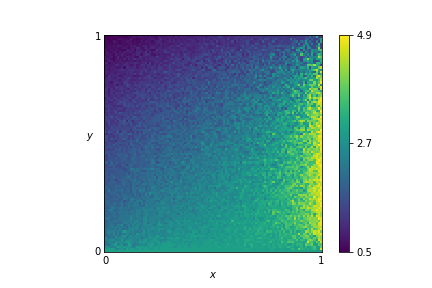
\includegraphics[height=.3\textheight]{src/chapters/02/img/Win-Stay_Lose-Shift.png}
    \caption{Pavlov fingerprinting with Tit for Tat used as the probe strategy.
    Figure was generated using~\cite{axelrodproject}.}
    \label{fig:fingerprinting}
\end{figure}

\begin{figure}[!hbtp]
    \centering
    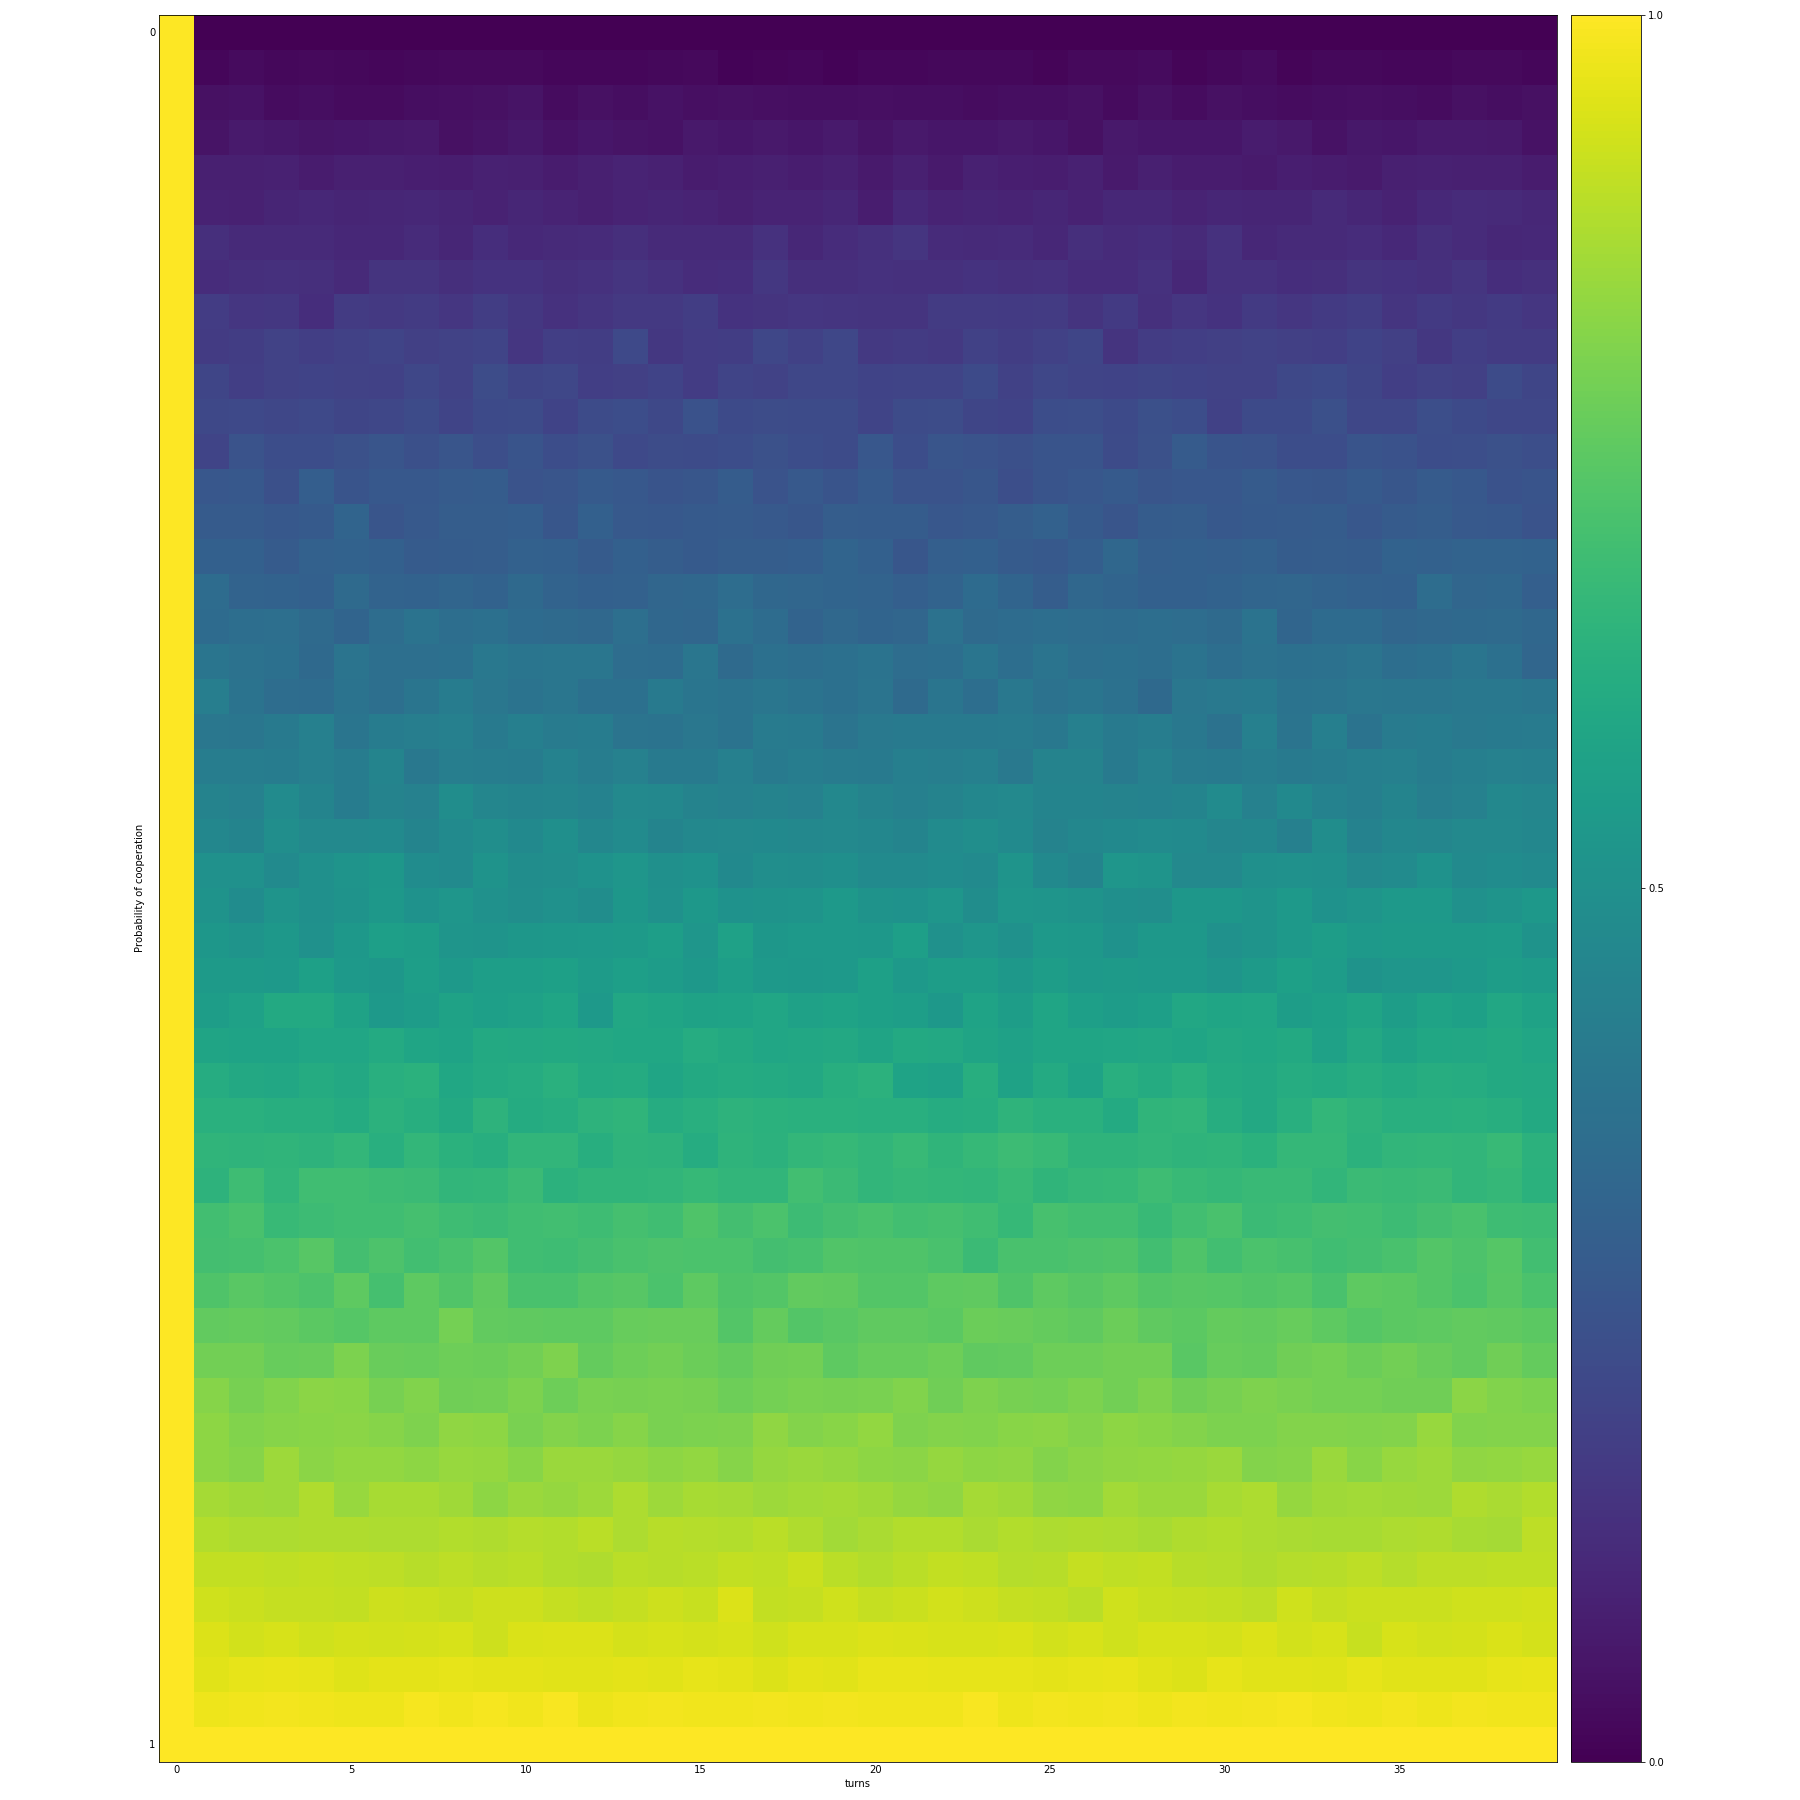
\includegraphics[height=.3\textheight]{src/chapters/02/img/Tit_for_Tat_fingerprint.png}
    \caption{Transitive fingerprint of Tit for Tat against a set of 50 random opponents.}
    \label{fig:transitive_fingerprinting}
\end{figure}

This section covered a series of structured strategies based on different
archetypes which have been trained via different training methods. The works
discussed on this sections have demonstrated that through these indirect
training processes successful IPD strategies can emerge. This thesis explores
both strategies of intelligent design (Chapter~\ref{chapter:memory_one}) and
trained strategies (Chapter~\ref{chapter:lstm})in more details. The next section
covers software that has been developed with the main aim of simulating the IPD
interactions.

\section{Software}\label{section:software}

Aside from human subject research the research of the IPD heavily relies on software.
This is to be expected as computer tournaments have become the main
means of simulating the interactions in an IPD game.
Many academic fields suffer from lack of source code availability and the IPD
is not an exception. Several of the tournaments that have been discussed so far were generated
using computer code, though not all of the source code is available.
The code for Axelrod's original tournament is known to be lost and
moreover for the second tournament the only source code available is the code
for the 62 strategies (found on Axelrod's personal website~\cite{fortan_code}).

Several projects, however, are open, available and have been used as research
tools or educational platforms over the years. Two such tools include
\cite{pd_trust} and~\cite{trust_blogb}.
The ``Game of Trust"~\cite{pd_trust} is an on-line, educational platform accessed 
through a graphical user interface,
for learning the basics of game theory, the IPD
and the notion of strategies. It attracted a lot of attention
due to being ``well-presented with scribble-y hand drawn
characters''~\cite{trust_blogb} and ``a whole heap of fun''~\cite{trust_bloga}.
Secondly,~\cite{pd_game} is a personal project written in PHP. It is a graphical user
interface that offers a big collection of strategies and allows the user to try
several matches and tournament configurations.

Open source projects used for research include~\cite{prison, axelrodproject}.
PRISON~\cite{prison} is written in the programming language Java and a
preliminary version was launched in 1998. It was used by its authors in several
publications, such as~\cite{Beaufils1997}, which introduced Gradual,
and~\cite{Beaufils1988}. The project includes a good number of strategies from
the literature, but unfortunately the last update of the project dates back to
2004. Axelrod-Python~\cite{axelrodproject} is a software used
in a number of works including~\cite{Knight2017,KnightHGC17, Goodman2018, Wang2017}. 
It is written in the
programming language Python following best practice
approaches~\cite{Aberdour2007, Benureau2018} and contains the largest collection
of strategies, known to the author. The strategy list of the project has been
cited by publications~\cite{Anastassacos2018, Hayes2017, Neumann2018}, and is
used in this thesis for Chapter~\ref{chapter:meta_tournaments} and
Chapter~\ref{chapter:best_response_sequence}.

\section{Chapter summary}

This Chapter presented a literature review of the Iterated Prisoner's
Dilemma. The opening sections focused on research trends and published works of
the field, followed by a presentation of research and educational software.
More specifically, Section~\ref{section:origin}
covered the early years of research. This was when simulating turns of the game
was only possible with human subject research.
Following the early years, the pioneering tournaments of Axelrod were introduced in
Section~\ref{section:intelligent_design}. Axelrod's work offered the field an
agent based game theoretic framework to study the IPD.
In his original papers he asked researchers to design strategies to test their
performance with the new framework. The winning strategy of both his tournaments
was Tit for Tat. The strategy however came with limitations which were explored
by other researchers, and new intelligently designed strategies were introduced in
order to surpass Tit for Tat with some contributions such as Pavlov and Gradual.

Soon researchers came to realise that strategies should not just do well in a tournament setting
but should also be evolutionary robust. Evolutionary dynamic methods were
applied to many works in the field, and factors under which cooperation
emerges were explored, as described in Section~\ref{section:evolutionary_dynamics}.
This was not done only for unstructured populations, where all strategies
in the population can interact with each other, but also in population where
interactions were limited to only strategies that were close to each other.
In such topologies it was proven that even in the one shot game, cooperation can
indeed emerge.

Evolutionary approaches can offer many insights in the study of the PD. In
evolutionary settings strategies can learn to adapt and take over population by
adjusting their actions; such algorithms can be applied so that evolutionarily
robust strategies can emerge. Algorithms and structures used to train strategies
in the literature were covered in Section~\ref{section:structured_strategies}.
From these training methods several strategies are found,
and to be able to differentiate between them fingerprinting was
introduced. The research of best play and cooperation has been going on since
the 1950s, and for simulating the game software has been developed along the
way. This software has been briefly discussed
in Section~\ref{section:software}.

The study of the PD is still an ongoing field research where new variants and
new structures of strategies are
continuously being explored~\cite{Ohtsuki2018}. The game now serves as a model
in a wide range of applications, for example in medicine and the study of cancer
cells~\cite{archetti2018, Kaznatchee2017}, as well as in social situations and
how they can be driven by rewards~\cite{Dridi2018}.
This thesis aims to contribute to the continued understanding of this well known
and widely applied game theoretic model.
Many of the papers reviewed in this Chapter have served as motivation to the
research presented in the following Chapters. In
Chapter~\ref{chapter:meta_tournaments} the performance of several of the
strategies mentioned in this Chapter is evaluated in a large number of
tournaments. Chapter~\ref{chapter:memory_one} explores the set of memory-one
strategies, and Chapters~\ref{chapter:best_response_sequence} and~\ref{chapter:lstm}
explore trained strategies based on archetypes such as sequences and recurrent
neural networks.
